%%%%%%%%%%%%%%%%%%%%%%%%%%%%%%%%%%%%%%%%%%%%%%%%%%%%%%%%%%%%%%%%%%%%%%%%%%%%%%%%%
% Introducción
%%%%%%%%%%%%%%%%%%%%%%%%%%%%%%%%%%%%%%%%%%%%%%%%%%%%%%%%%%%%%%%%%%%%%%%%%%%%%%%%%

\chapter{Estado del arte} % (fold)
\label{sec:EstadoDelArte}

    %%% Más cosas por aquí estaría bien, primero hay que entender que es Estado del Arte :)

    \section{Opciones actuales en el mercado} % (fold)
    \label{sec:OpcionesActualesEnElMercado}

        Son múltiples las baterías electrónicas a la venta. Una búsqueda rápida en Thomann\cite{thomann_baterias} nos
        muestra una gran variedad de baterías electrónicas en un amplío rango de precios, desde los 109\euro{} hasta los
        8.398\euro{}.

        \begin{figure}[ht]
            \centering
            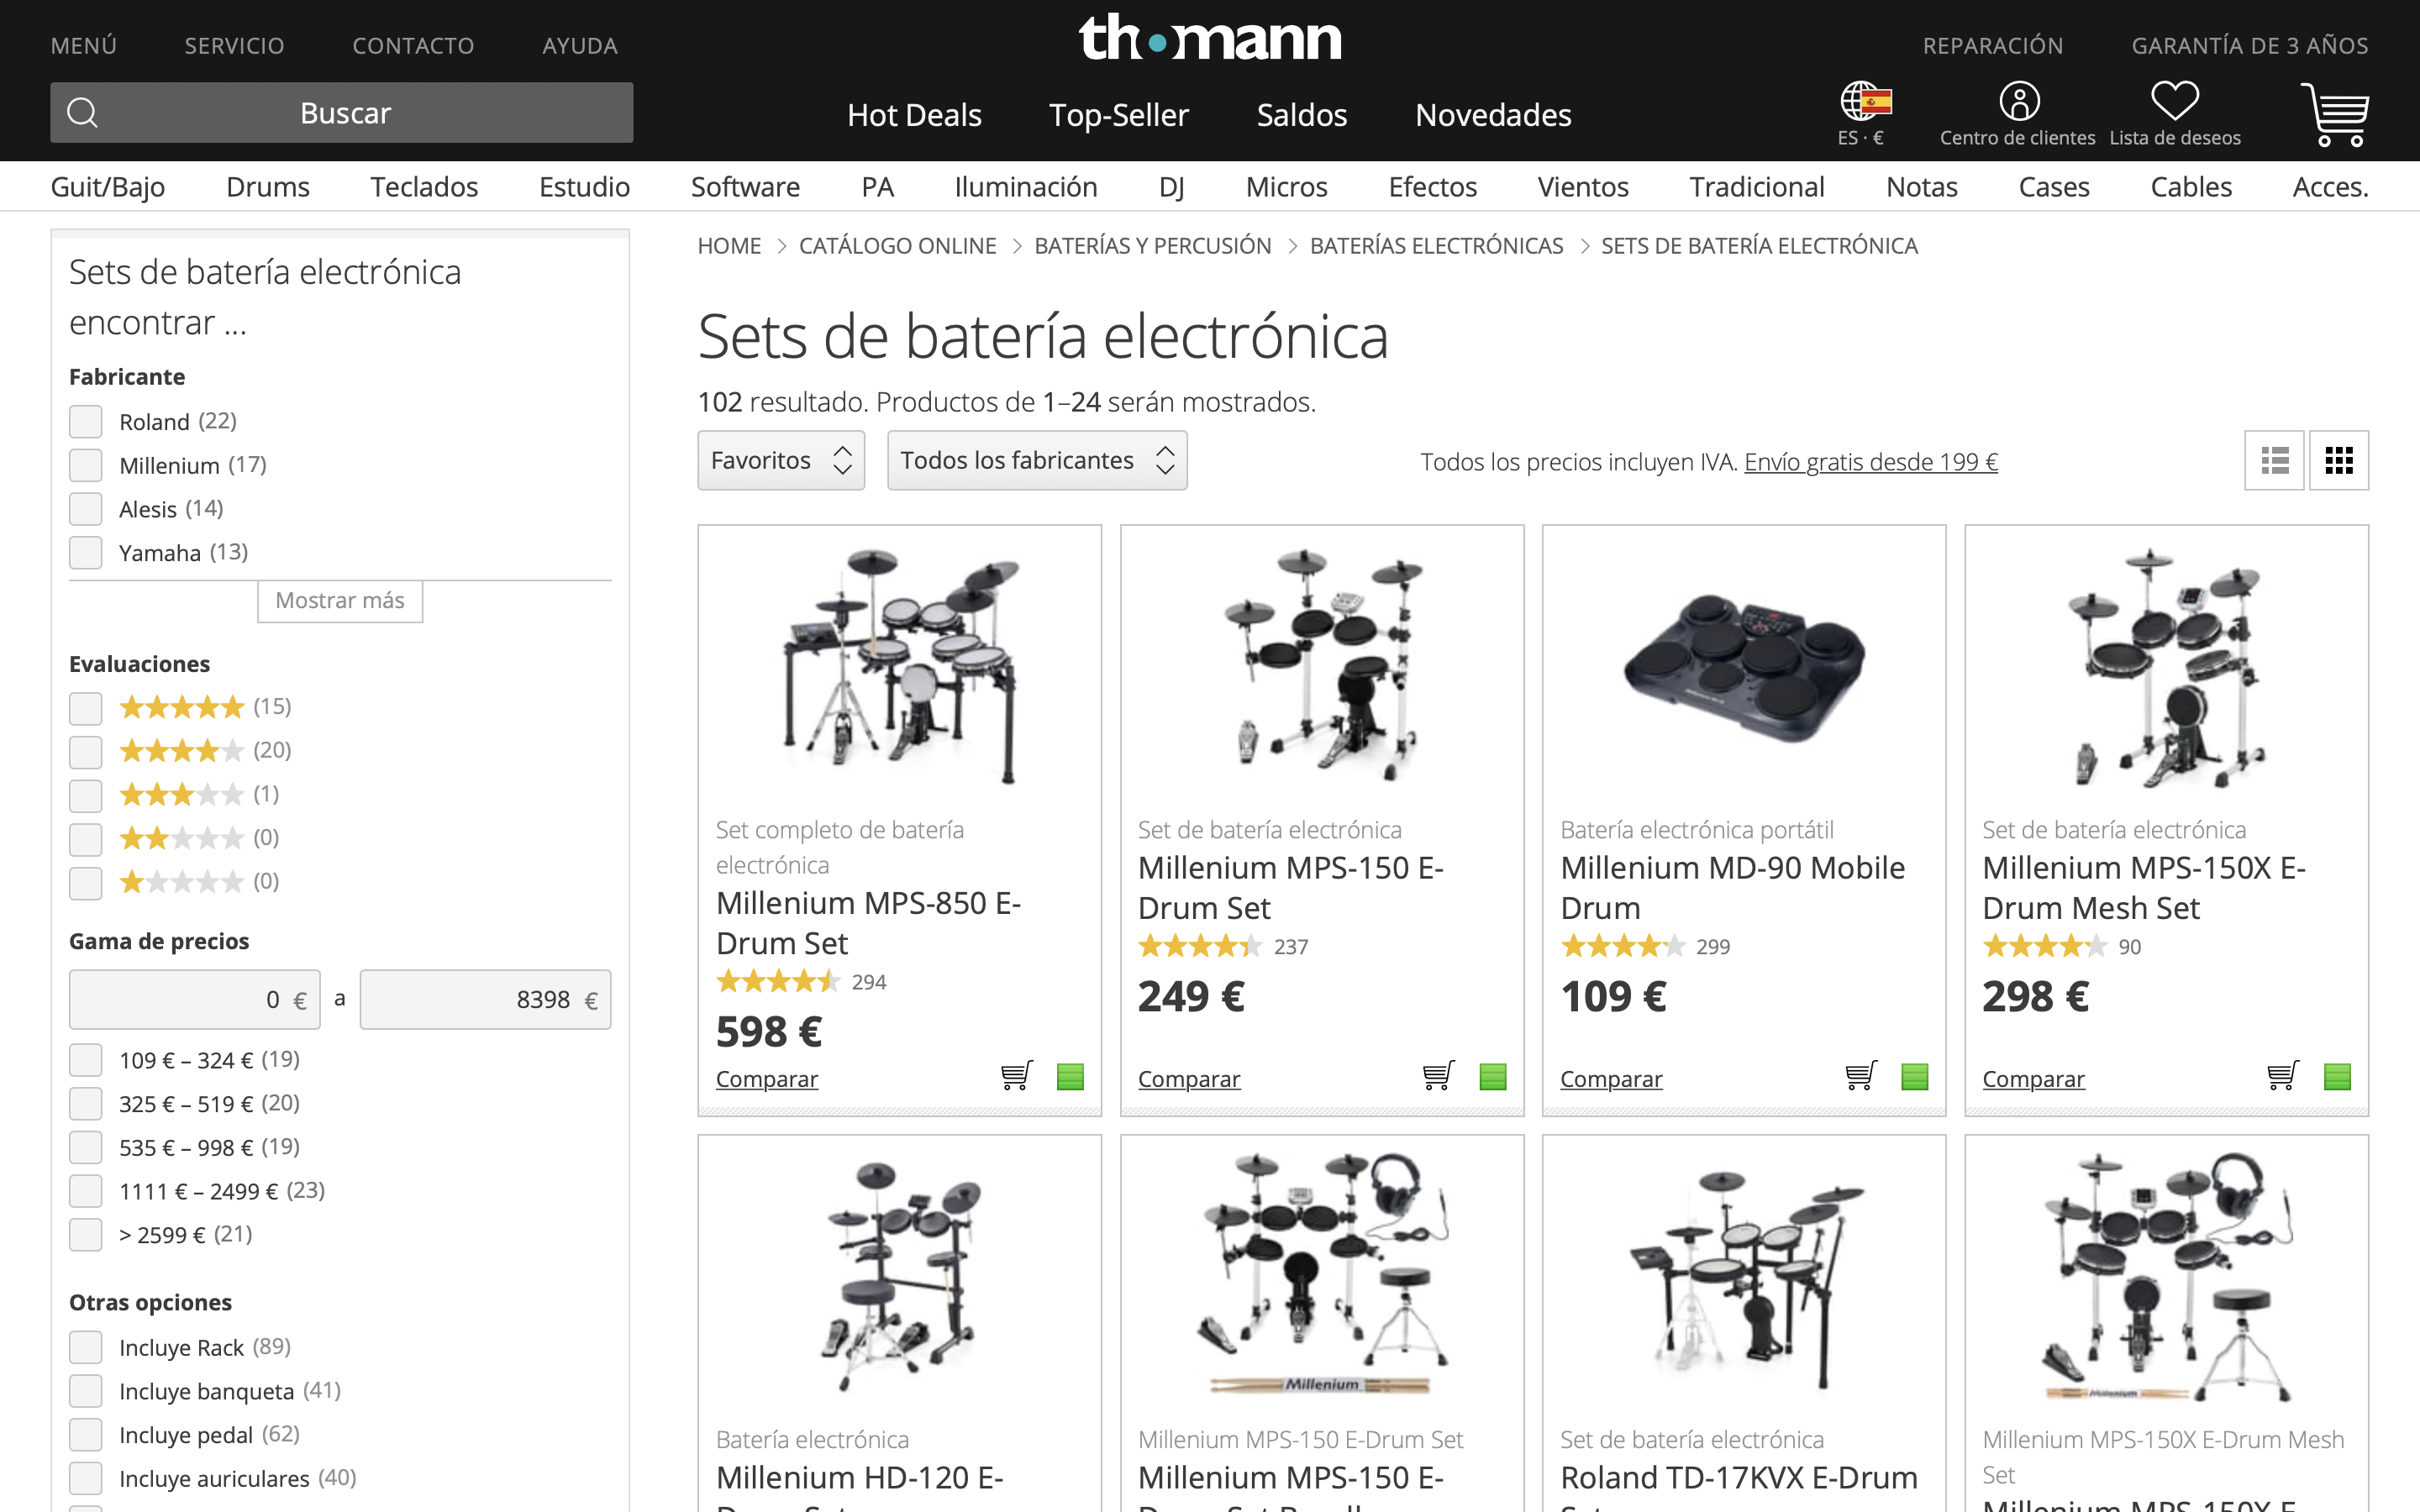
\includegraphics[width=\textwidth]{thomann_baterias}
            \caption{Resultados de la búsqueda de baterías electrónicas en Thomann}
        \end{figure}

        En el terreno del código abierto, %%%%%%%%%%%%%% cosas
    
    % section Opciones actuales en el mercado (end)

    \section{Propuesta} % (fold)
    \label{sec:Propuesta}

        La propuesta que se presenta es un crear un programa de código abierto para que cualquier persona con unos
        conocimiento medios de informática pueda montar su propia batería electrónica en casa.
        
        Para completar con éxito el objetivo de este proyecto, los puntos más importantes serán:
        \begin{itemize}
            \item Reproducción del sonido con el menor delay posible.
            \item Reproducción de varios sonidos al mismo tiempo.
            %%%%%%%%%%%%%%%%%%%%%%%%%%%%%%%%%%%%%%%%%%%%%%%%%%%%%%
        \end{itemize}
    
    % section Propuesta (end)

% chapter Estado del arte (end)
